% Data used by each group of strategies in the binary study: the estimator's
% training share, the tuning share and the common test set.
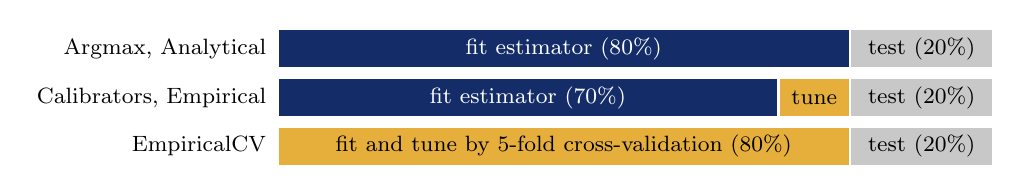
\begin{tikzpicture}[x=.075\textwidth, y=.62cm, font=\footnotesize,
    seg/.style={draw=white, line width=1pt, minimum height=.5cm,
      inner sep=0pt, anchor=west},
    rowlbl/.style={anchor=east, align=right}]
  \definecolor{splitfit}{HTML}{142D69}
  \definecolor{splittune}{HTML}{E6AF3C}
  \definecolor{splittest}{HTML}{C8C8C8}
  % Row 1: no tuning.
  \node[rowlbl] at (0, 2) {Argmax, Analytical};
  \node[seg, fill=splitfit, text=white, minimum width=.6\textwidth]
    at (0, 2) {fit estimator ($80\%$)};
  \node[seg, fill=splittest, minimum width=.15\textwidth]
    at (8, 2) {test ($20\%$)};
  % Row 2: single validation split.
  \node[rowlbl] at (0, 1) {Calibrators, Empirical};
  \node[seg, fill=splitfit, text=white, minimum width=.525\textwidth]
    at (0, 1) {fit estimator ($70\%$)};
  \node[seg, fill=splittune, minimum width=.075\textwidth]
    at (7, 1) {tune};
  \node[seg, fill=splittest, minimum width=.15\textwidth]
    at (8, 1) {test ($20\%$)};
  % Row 3: cross-validation over the training pool.
  \node[rowlbl] at (0, 0) {EmpiricalCV};
  \node[seg, fill=splittune, minimum width=.6\textwidth]
    at (0, 0) {fit and tune by $5$-fold cross-validation ($80\%$)};
  \node[seg, fill=splittest, minimum width=.15\textwidth]
    at (8, 0) {test ($20\%$)};
\end{tikzpicture}
